%
%
%
\section{Spatial Discretisation}
\label{space_discretisation_nl.sec}
\headb{Nonlinear Navier-Stokes solver}{Spatial discretisation}
%
 The development of a FV edge-based data structure
 for unstructured mixed-element meshes
 will now be described in detail.

%
\begin{figure}[ht]
\centerline{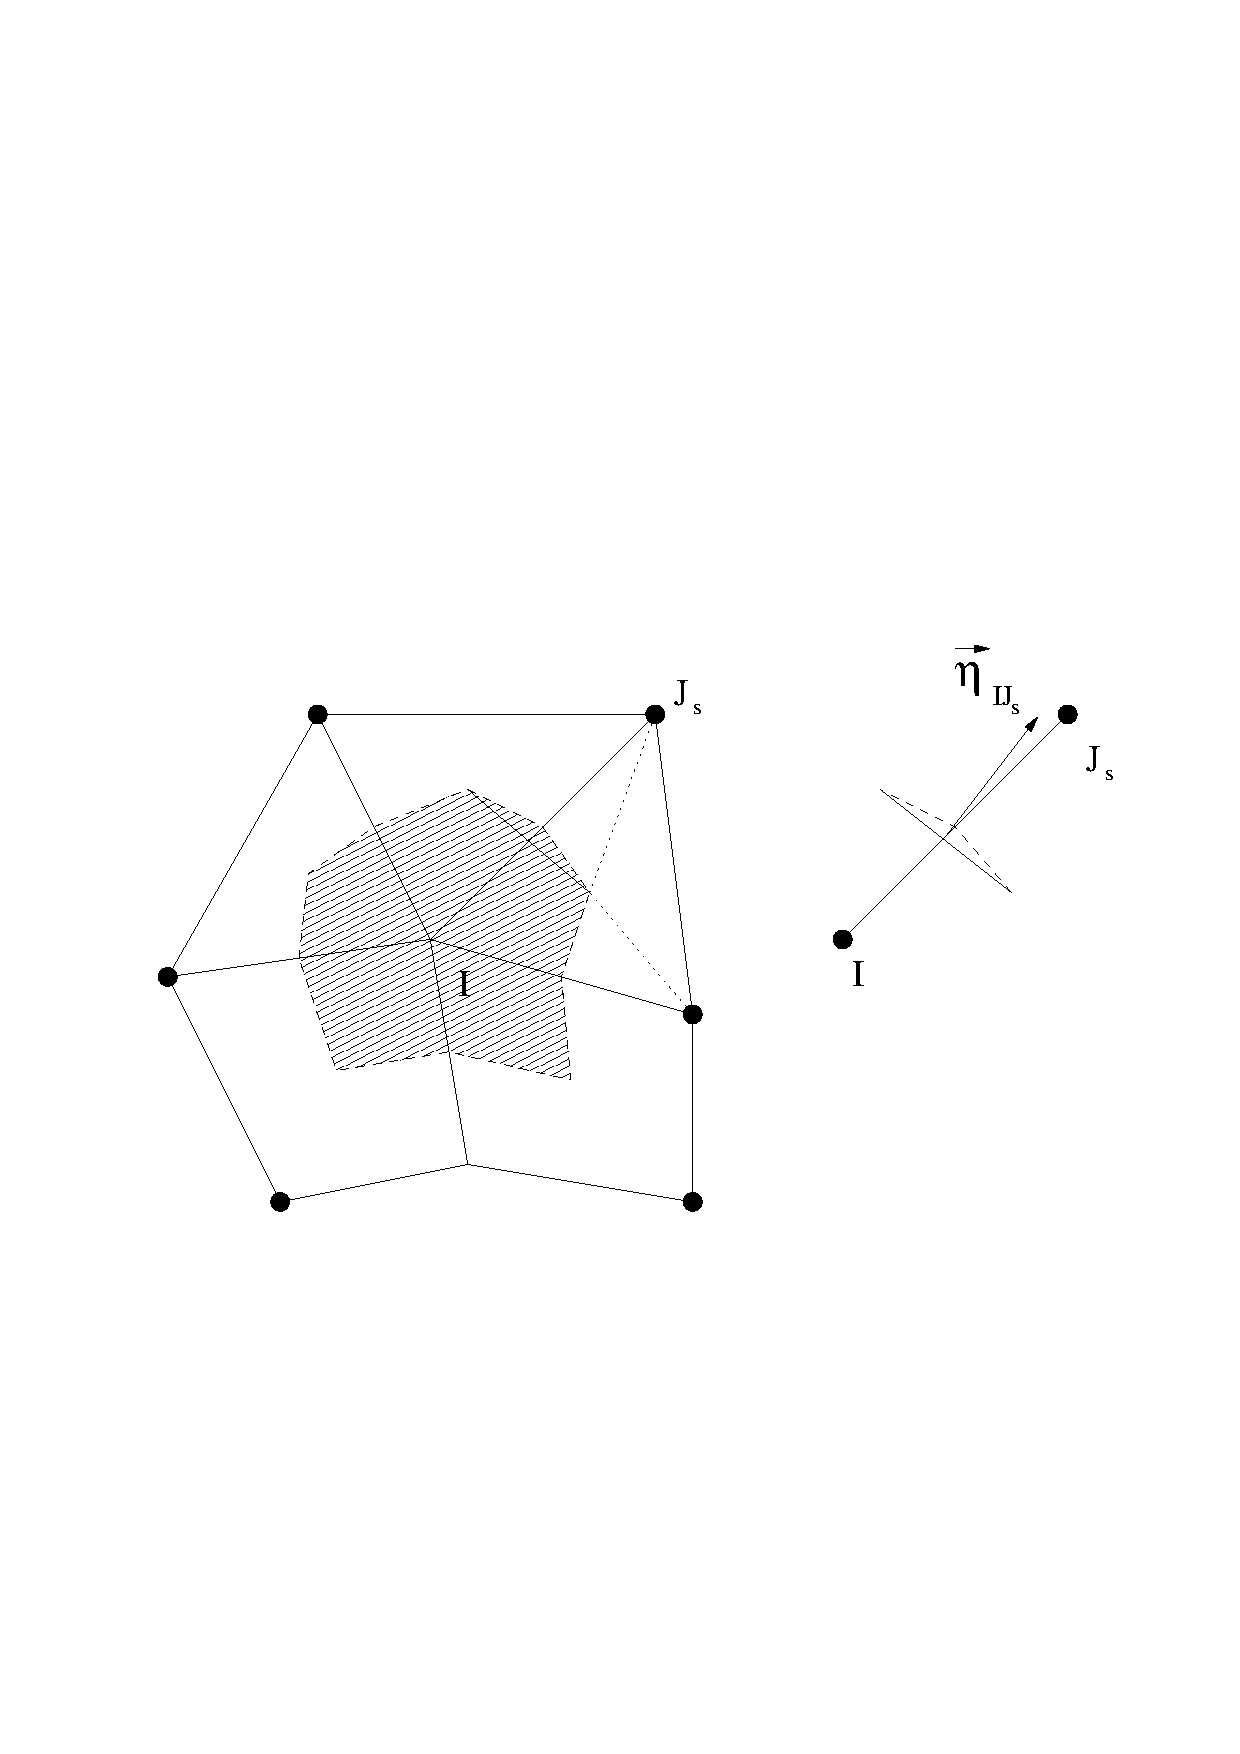
\includegraphics[width=80mm,clip=t]{CHAP_NONLIN/FIGURE/mixme.pdf}}
\caption{Control volume for node $I$ and metric vector
$\vec{\eta}\sm{IJs}$
 for edge $IJs$}
\label{median_dual.fig}
\end{figure}
%
 As shown for the 2D mesh of Fig. \ref{median_dual.fig},
 using a node-centered approach and choosing the median dual mesh as control
 volume\footnote{A discussion of different control volume definitions is
 given by Barth \& Jespersen 1989.},
 a FV discretisation of
 (\ref{conservative_formulation_nl.eq}), written
 in a semi-discrete form, is given by:

%
\beq
  \fpdt{\left({\cal V}\sm{I}{\bf U}\sm{I}\right)} &=& -\!
  \sum\sm{s=1}\se{m\sm{I}} \left[\left|\vec{\eta}\sm{IJs}\right|
  \left({\cal F}\sm{IJs}\!-\!{\cal G}\scriptstyle{m}\sm{IJs}\right)
  - \tau\sm{IJs} {\cal G}\scriptstyle{l}\sm{IJs}\right]
  + {\cal V}\sm{I}{\bf S}\sm{I}
  \label{semi_discrete_nl.eq}
\eeq
%
 As shown in Fig. \ref{median_dual.fig}, node $I$ is connected by edges to
 $m\sm{I}$ ($m\sm{I} = 6$ in Fig. \ref{median_dual.fig})
 nodes $J\sm{s}$, ${\cal V}\sm{I}$ representing the control volume
 associated with it.
 ${\cal F}$, ${\cal G}\scriptstyle{m}$ and ${\cal G}\scriptstyle{l}$
 correspond to the inviscid and viscous vectors $\vec{\bf F}$,
 $\vec{\bf G}\scriptstyle{m}$ and $\vec{\bf G}\scriptstyle{l}$.
 $\vec{\eta}\sm{IJs}$ is the metric vector associated with the
 surface area of edge $IJs$ while $\tau\sm{IJs}$ represents the Laplacian
 weight associated with the same edge.
 The summation in (\ref{semi_discrete_nl.eq}) has been obtained applying
 the Green's formula to the surface integral of (\ref{conservative_formulation_nl.eq})
 and choosing as path the median dual mesh (Barth \& Jespersen \citeyearNP{Barth:1},
 Barth \citeyearNP{Barth:2}).
 Of particular interest here is the use of the GFE node-pair formula
 for the Laplacian operator $\tau\sm{IJs}$ in order to construct
 an approximate version for the FV edge-data scheme
 (Sbardella \& Imregun \citeyearNP{Luca:7,Luca:11}).
%
%
%
%
%
\subsection{Inviscid discretisation}
\label{inviscid_disretisation.subsec}
%
 The discretisation of the inviscid flow terms in
 (\ref{semi_discrete_nl.eq}) is given by:

%
\beq
  \sum\sm{s=1}\se{m\sm{I}} \left|\vec{\eta}\sm{IJs}\right|
  {\cal F}\sm{IJs}
 \label{inviscid_contribution_nl.eq}
\eeq
%
 where ${\cal F}\sm{IJs}$ represents the inviscid flux function along edge
 $IJ\sm{s}$
 which is obtained using a central difference scheme with added
 matrix artificial dissipation. This artificial dissipation
 is a blend of second and fourth order differences. The fourth order
 terms ensure the stability of the scheme in smooth regions of the flow,
 while the second order terms are required to damp numerical oscillations
 in the vicinity of discontinuities.
 The inviscid flux function is expressed as:

%
\beq
  {\cal F}\sm{IJs} = \frac{\vec{\bf F}\sm{I}+\vec{\bf F}\sm{Js}}{2}
  \cdot\frac{\vec{\eta}\sm{IJs}}{\left|\vec{\eta}\sm{IJs}\right|}
  - {\cal D}\sm{IJs}
  \label{inviscid_flux_function_nl.eq}
\eeq
%
 where the artificial dissipation ${\cal D}\sm{IJs}$ along the edge is
 given by:

%
\beq
  {\cal D}\sm{IJs} = \frac{1}{2}
  \left|{\bf A}\sm{IJs}\right|
  \left[\psi\Delta{\bf U} - \epsilon\sm{4}\left(1-\psi\right)\Delta{\cal L}\left({\bf U}\right)\right]
  \label{artifical_diffusion_nl.eq}
\eeq
%
 Here $\Delta$ represents the difference operator along edge $IJs$

%
\beq
  \Delta\left(\cdot\right) = \left(\cdot\right)\sm{Js} -
\left(\cdot\right)\sm{I}
\label{difference_operator.eq}
\eeq
%
 $\left|{\bf A}\sm{IJs}\right|$ is the standard Roe matrix
 (Roe \citeyearNP{Roe:1})
 between the two stages ${\bf U}\sm{I}$ and ${\bf U}\sm{Js}$,
 $\epsilon\sm{4}\approx 1/16$ is the fourth order artificial dissipation
 coefficient. $\cal L\sm{I}\left({\bf U}\right)$ is a pseudo-Laplacian
 operator, at node $I$, given by:

%
\beq
  {\cal L}\sm{I}\left({\bf U}\right) =
  \left(\sum\sm{s=1}\se{m\sm{I}}
  \frac{{\bf U}\sm{Js}-{\bf U}\sm{I}}{s\sm{IJs}}\right)
  \left(\sum\sm{s=1}\se{m\sm{I}}
  \frac{1}{s\sm{IJs}}\right)\se{-1}
  \label{pseudo_lapl_nl.eq}
\eeq
%
 where

%
\beq
  s\sm{IJs} = \left|\vec{x}\sm{Js} - \vec{x}\sm{I}\right|
  \label{svalll.eq}
\eeq
%
 $\psi$ represents the limiter function which varies between
 0 and 1 and it is required in order to switch the scheme to first order
 ($\psi = 1$) in the vicinity of discontinuities (Jorgenson \&
 Turkel \citeyearNP{Turkel:2}).
%
%
\subsubsection{Evaluation of metric vector}
%
 The metric vector $\vec{\eta}\sm{IJs}$ is obtained
 via a summation of the two dual median lengths around the edges,
 multiplied by their normals. For example the metric vector of the edge
 connecting nodes $I$ and $Js$ is shown in Fig. \ref{median_dual.fig} for a
 2D mesh.
 Another way of calculating $\vec{\eta}\sm{IJs}$ is the use of the
 GFE scheme in a node-pair formulation
 (Selmin \& Formaggia \citeyearNP{Formaggia}):

%
\beq
  \vec{\eta}\sm{IJs} = \sum_{e \in IJs} \int\sm{{\cal V}\sm{e}}
  \left(N\sm{I}\nabl N\sm{Js} - N\sm{Js}\nabl N\sm{I}\right) d{\cal V}
  \label{inviscid_weigh.eq}
\eeq
%
 where $e \in IJs$ indicates the set of elements which
 share nodes $I$ and $Js$, and $N\sm{I}$ is the test function of
 the GFE method.
 In the derivation of (\ref{inviscid_weigh.eq}), no a-priori assumptions
 were made regarding element types or the space dimensionality of the flow.
 If the FE test function $N$ is linear,
 both FV and GFE schemes will result in the same neighbouring stencil
 on triangular and tetrahedral meshes.
 Since all nearest neighbours are joined to the vertex under consideration
 by an edge, the node-pair formulation
 of (\ref{inviscid_weigh.eq}) is equivalent to an edge-based data
 structure (Bath \& Jespersen \citeyearNP{Barth:1},
 Selmin \& Formaggia \citeyearNP{Formaggia}).
%
\begin{figure}[ht]
 \begin{center}
  \begin{tabular}{cc}
    \subfigure[Galerkin finite element (GFE)]
     {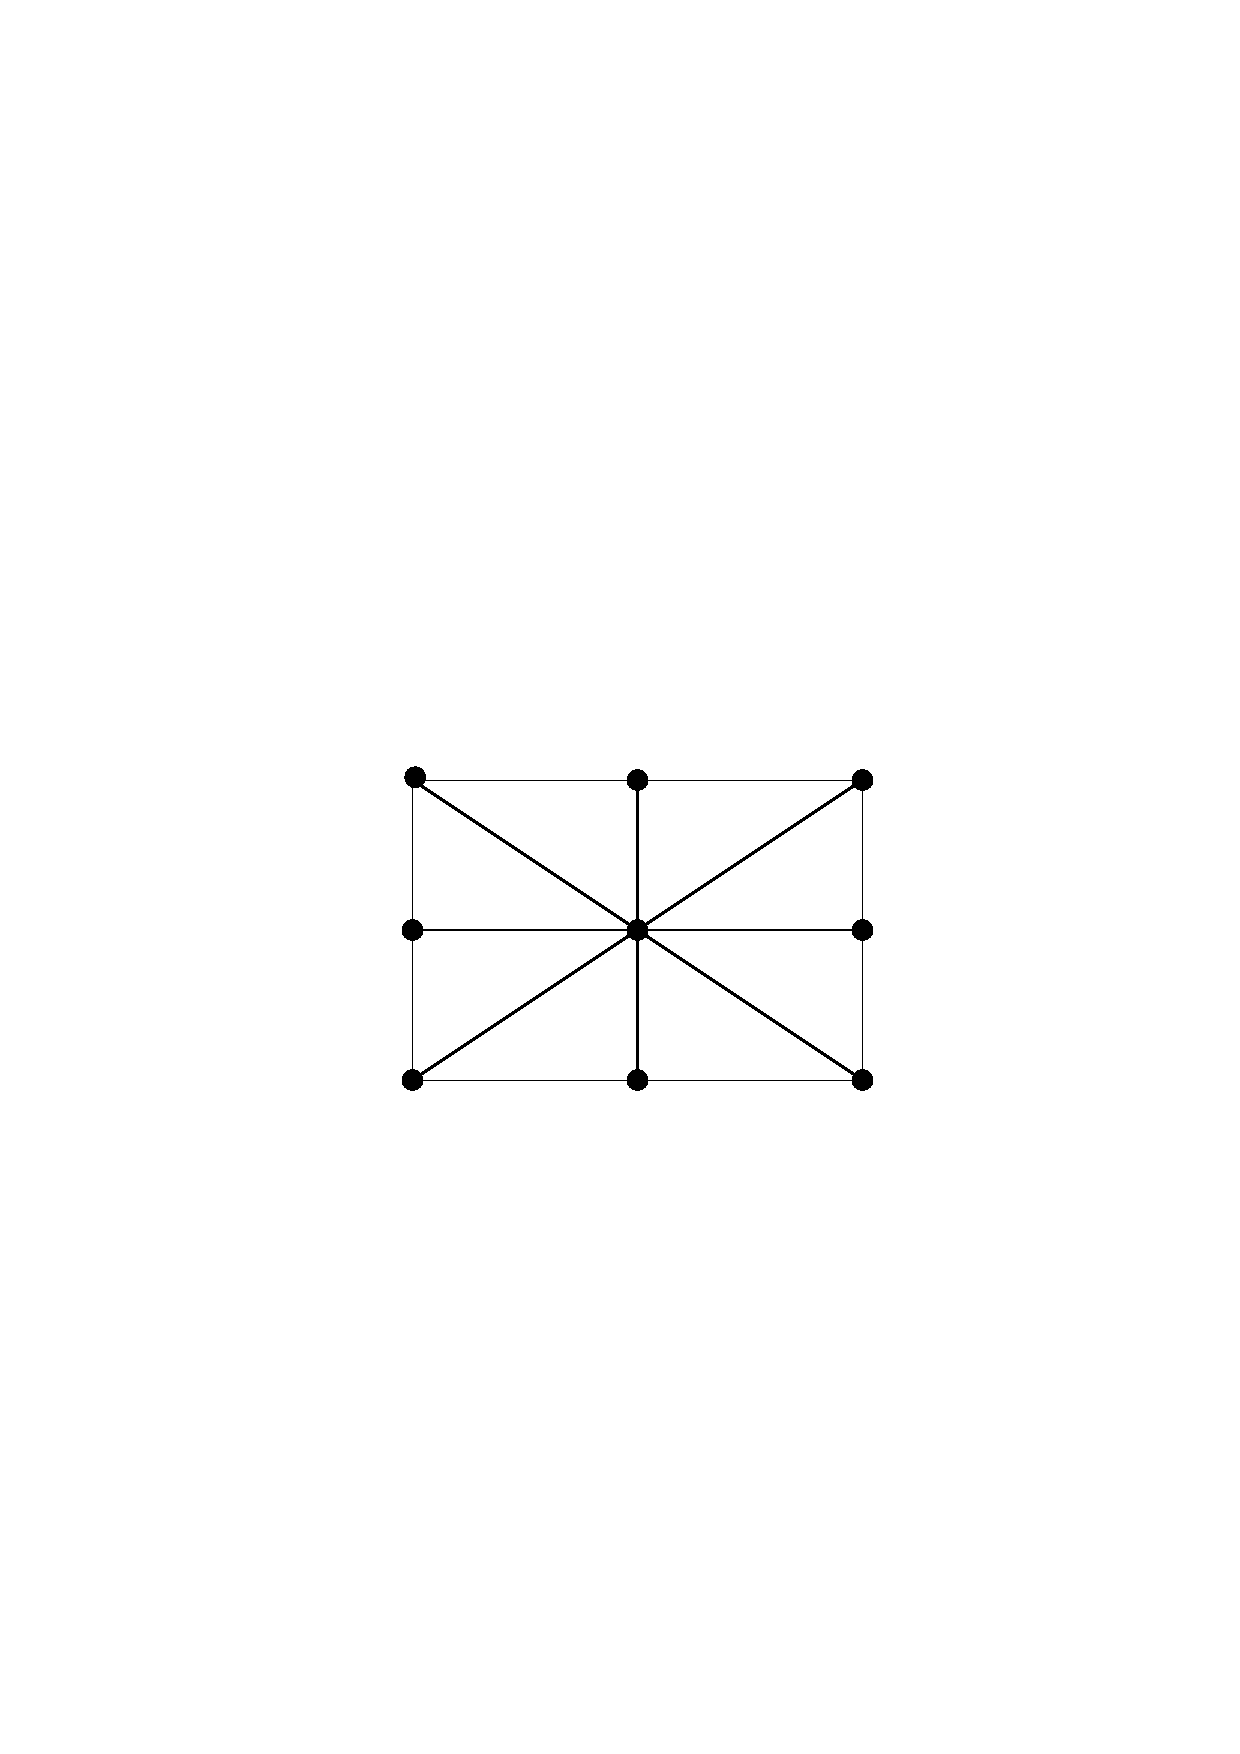
\includegraphics[width=60mm,clip=t]{CHAP_NONLIN/FIGURE/fe_quad_stencil.pdf}}
     &
    \subfigure[Finite volume (FV)]
     {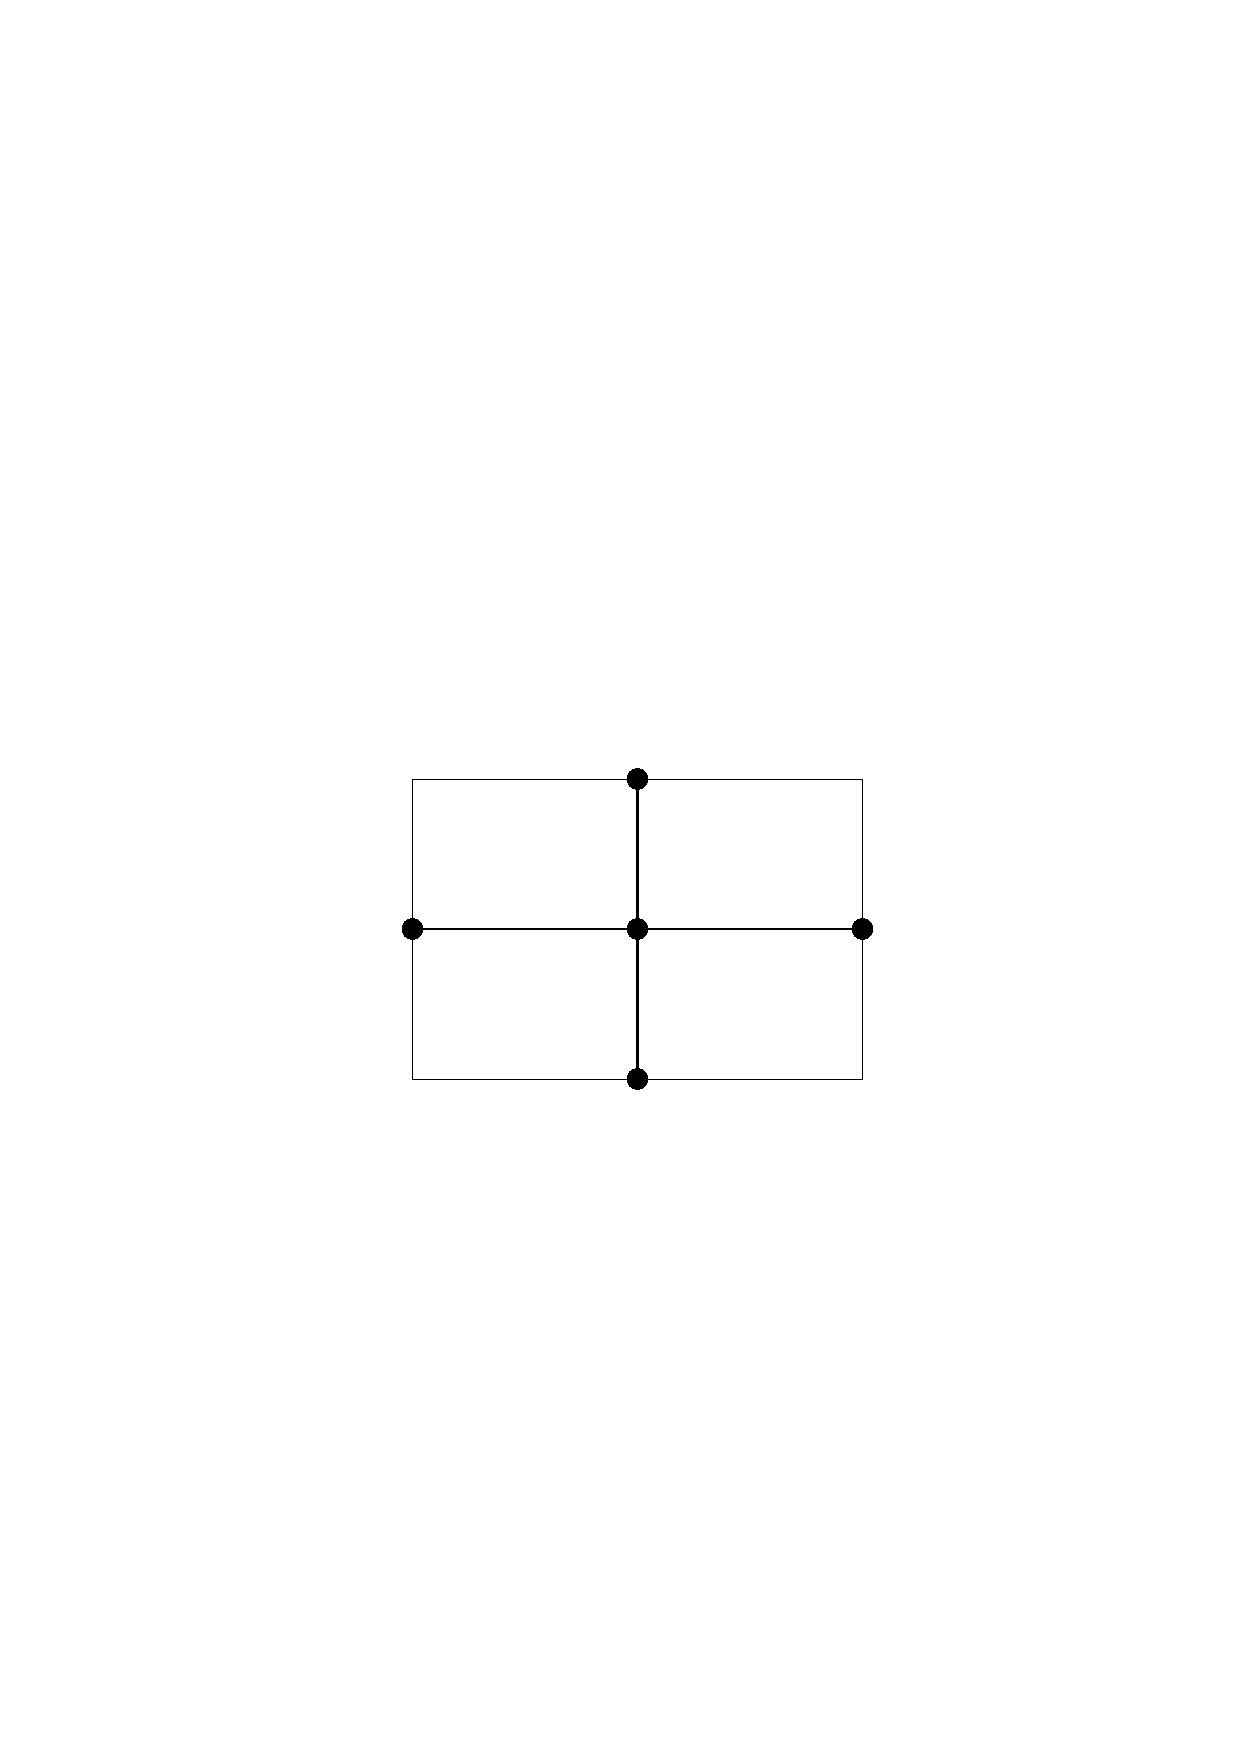
\includegraphics[width=60mm,clip=t]{CHAP_NONLIN/FIGURE/fv_quad_stencil.pdf}}
   \end{tabular}
  \end{center}
\vspace{-5mm}
\caption{Stencils for a quadrilateral mesh}
\label{fe_fv_quadrilateral.fig}
\end{figure}
%
 However, for quadrilaterals in 2D, and pyramids, wedges
 and hexahedra in 3D,
 the edge-data structure of a standard FV discretisation
 is no longer equivalent to the node-pair formulation of the GFE
 method.
 For example, in the case of a quadrilateral element, the GFE formulation
 takes into account the diagonal links. This approach results
 in a 9-point stencil, involving all corner points of the 4 quadrilaterals
 which share the vertex under consideration.
 On the other hand, the classical FV formulation considers the edge-based
 links only, resulting in a 5-point stencil (Fig. \ref{fe_fv_quadrilateral.fig}).
 Similarly, for a hexahedral element, the GFE method results in a 27-point
 stencil whereas the FV results in a 9-point stencil.
 Consequently, the GFE method is more expensive than the standard FV method
 but it has less dependence on mesh quality. For instance, when a mesh
 of quadrilateral or hexahedral elements is not orthogonal,
 the FV scheme still retains its conservation properties but its accuracy
 degenerates from second to first order (Essers at al. \citeyearNP{Essers:1}).
 For distorted meshes,
 the FV scheme is unable to recover the correct
 gradient values for a linear field on such elements. However, in the present
 formulation, the gradient information is used only
 for the evaluation of the limiter $\psi$
 in (\ref{artifical_diffusion_nl.eq}).
 By adopting a suitable limiter function, as that developed by Jorgenson \&
 Turkel \citeyear{Turkel:2},
 the FV scheme should retain its overall second order accuracy.
%
%
\subsubsection{Artificial dissipation and limiter function}
%
 Central-difference type schemes, such that in (\ref{inviscid_flux_function_nl.eq}),
 are commonly used for the solution of the Euler and Navier-Stokes equations.
 The artificial dissipation ${\cal D}\sm{IJs}$ in (\ref{artifical_diffusion_nl.eq})
 plays a crucial role in the determination of the quality of the numerical method.
 One of the first central-difference schemes used the
 scalar artificial dissipation model developed by Jameson et at.
 \citeyear{Jame:1}. During the 1980s, a considerable amount of research effort
 has been devoted towards the construction of more sophisticated
 schemes by minimising the added artificial dissipation.
 The paper by Swanson \& Turkel \citeyear{Turkel:1} summarises
 such effort and shows how central difference schemes
 with matrix artificial dissipation, as that in (\ref{artifical_diffusion_nl.eq}),
 are related to upwind schemes which utilize concepts from the characteristic
 theory in order to determine the direction of spatial differencing
 (Roe \citeyearNP{Roe:1}, Harten \citeyearNP{Harten:2}, Osher \citeyearNP{Osher:1},
 Pandolfi \citeyearNP{Pandolfi}, Roe \citeyearNP{Roe:2}).
 In fact, scheme (\ref{inviscid_flux_function_nl.eq}) with $\psi = 1$
 is equivalent to the first-order upwind scheme of Roe \citeyear{Roe:1}.
 Also, upwind schemes can be designed to have the TVD property
 in the case of scalar conservation laws
 (Harten \citeyearNP{Harten:1}, Osher \citeyearNP{Osher:2}).
 The TVD property is very useful in constructing limiter functions
 for second-order numerical schemes (Sweby \citeyearNP{Sweby:1}).
 Swanson \& Turkel \citeyear{Turkel:1} introduced flux limiter functions
 that are consistent with the central-difference dissipation models using the TVD
 property.

 The limiter function used here is a multidimensional extension
 of the modified, van Leer central difference limiter, proposed
 by Swanson \& Turkel \citeyear{Turkel:1}. For an equispaced
 1D mesh, the limiter function at point $I$ is defined as:

%
\beq
  \psi\sm{I} = \frac{\left|p\sm{I+1}-2 p\sm{I} + p\sm{I-1}\right|}
               {\left(1-\chi\right)\left(\left|p\sm{I+1}-p\sm{I}\right|+
                                     \left|p\sm{I}-p\sm{I-1}\right|\right)+
                         \chi\left(p\sm{I+1}+2 p\sm{I} + p\sm{I-1}\right)}
  \label{limiter.eq}
\eeq
%
 where $0 \leq \chi \leq 1$. If $\chi = 0$, $\psi\sm{I}$ becomes
 the van Leer central difference TVD limiter. If $\chi = 1$,
 $\psi\sm{I}$ is equivalent to that used  by Jameson et al.  \citeyear{Jame:1}.
 For a 3D mesh the limiter function associated with node $I$
 and side $IJs$ becomes:

%
\beq
  \left.\psi\sm{I}\right|\sm{IJs} =
  2\frac{\left| p\sm{Js} - p\sm{I} - \nabl p\sm{Js}\cdot\vec{s}\sm{IJs}\right|}
  {\left(1-\chi\right)
   \left(\left|p\sm{Js}-p\sm{I}\right|+
         \left|p\sm{I}-p\sm{Js}+\nabl p\sm{Js}\cdot\vec{s}\sm{IJs}\right|\right)
   + 2\chi\left(p\sm{Js}+p\sm{I}\right)}
  \label{limiter_mult_1.eq}
\eeq
%
 where $\vec{s}\sm{IJs}$ is given in (\ref{svalll.eq}).
 The final value of $\psi\sm{I}$ is than given by the maximum value
 of (\ref{limiter_mult_1.eq}) of all sides $IJs$ associated with node $I$:
%
\beq
  \psi\sm{I} = {\tt max}\left(\left.\psi\sm{I}\right|\sm{IJs}\right)
  \label{limiter_mult_2.eq}
\eeq
%
 The central-difference scheme in (\ref{inviscid_flux_function_nl.eq})
 is slightly more dissipative than a second-order upwind scheme and this
 is for two reasons. First
 $\psi\sm{I} = {\tt max}\left(\left.\psi\sm{I}\right|\sm{IJs}\right)$,
 is multidirectional, while $\psi\sm{I}$ is usually chosen along a particular
 direction in upwind schemes.
 Second, upwind limiters allow to have negative viscosity
 but still retaining the TVD property while central-difference scheme cannot
 have negative artificial dissipation.
 In any case, to compensate for this slight increase in dissipation,
 central-difference schemes are simpler to program and require
 less computer time per time step, especially if used in conjunction with
 multistage time stepping techniques where the artificial dissipation
 is evaluated at alternate stages (Appendix \ref{multigrid.chap}).
%
%
%
%
%
%
\subsection{Viscous discretisation}
\label{viscous_disretisation.subsec}
%
 The viscous fluxes associated with the mixed derivatives in
 $\vec{\bf G}\sm{m}$ of (\ref{mean_flow_mixed.eq})
 are treated in the same way as their inviscid
 counterparts and their contribution to (\ref{semi_discrete_nl.eq}) is given by:

%
\beq
  {\cal G}{\scriptstyle m}\sm{IJs} =
  \frac{1}{Re}\left(\vec{\bf G}{\scriptscriptstyle m}\sm{I} +
  \vec{\bf G}{\scriptscriptstyle m}\sm{Js}\right)\cdot
  \frac{\vec{\eta}\sm{IJs}}{\left|\eta\sm{IJs}\right|}
  \label{viscous_mix_nl.eq}
\eeq
%
 Here, the Laplacian terms will be treated in a novel way in order to
 improve both the accuracy and the robustness of the numerical scheme
 (Sbardella \& Imregun \citeyearNP{Luca:11}).
 In (\ref{semi_discrete_nl.eq}), these terms take the form:

%
\beq
 {\cal G}\scriptstyle{l}\sm{IJs} =
 \frac{1}{Re}\left[
 \begin{array}{c}
  0 \\ \mu\sm{IJs} \Delta v\sm{1}
    \\ \mu\sm{IJs} \Delta v\sm{2}
    \\ \mu\sm{IJs} \Delta v\sm{3}
    \\ \left(\mu \vec{v}\right)\sm{IJs}\cdot \Delta \vec{v} +
       +
\frac{\gamma}{\gamma\!-\!1}\left(\frac{\mu\sm{l}}{Pr\sm{l}}\!+\!
         \frac{\mu\sm{l}}{Pr\sm{t}}\right)\sm{IJs}\Delta T
 \end{array}
 \right]
 \label{bbbbbbbb.eq}
\eeq
%
 The subscript $IJs$ indicates an arithmetic mean over nodes $I$ and $Js$:
%

\beq
  \left(\cdot\right)\sm{IJs} =
  \frac{\left(\cdot\right)\sm{Js}+\left(\cdot\right)\sm{I}}{2}
  \label{side_average.eq}
\eeq
%
 The difference operator $\Delta$ in (\ref{bbbbbbbb.eq})
 is given in (\ref{difference_operator.eq}).
 In the present formulation, that deals with mixed-element meshes, the
 Laplacian weight $\tau\sm{IJs}$ in (\ref{semi_discrete_nl.eq}) is evaluated using
 an approximation of the GFE node-pair relation.
 For a generic 2D or 3D element, the GFE Laplacian weight can be written as
 (Selmin \& Formaggia \citeyearNP{Formaggia}):

%
\beq
  \tau\sm{IJs} = -\sum\sm{e\in IJs} \int\sm{{\cal V}\sm{e}}
  \nabl N\sm{I}\cdot\nabl N\sm{Js} d{\cal V}
  \label{laplacian_coefficient.eq}
\eeq
%
 As for (\ref{inviscid_weigh.eq}), the Laplacian node-pair coefficient
 can be used for triangle/tetrahedral elements only if the data structure
 is edge based.
 Equation (\ref{laplacian_coefficient.eq}) will now be extended to other types
 of elements so that an approximate Laplacian weight, that is suitable for an edge-data
 FV implementation, can be evaluated.
 Let us consider the quadrilateral element of Fig. \ref{laplacian.fig} to
 illustrate such an approach.
%
\begin{figure}[ht]
\centerline{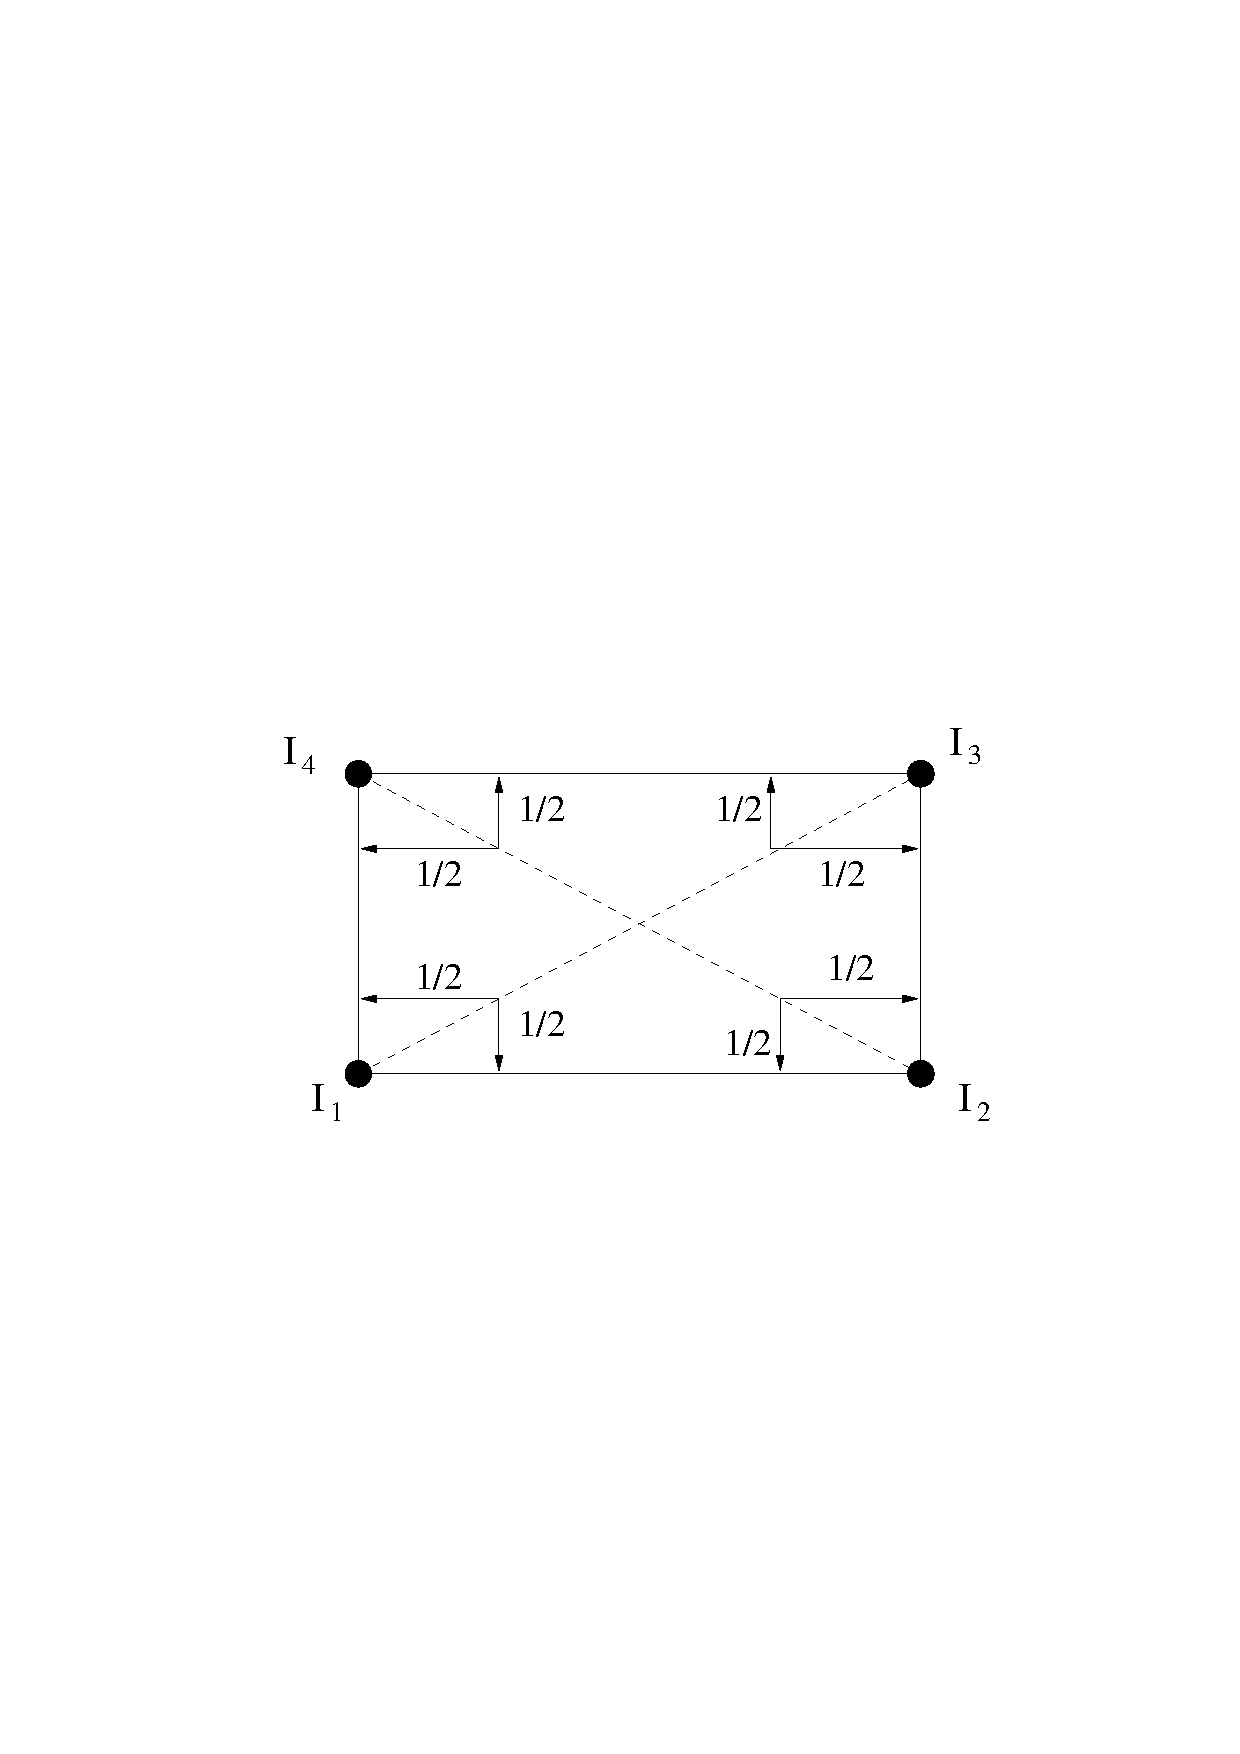
\includegraphics[width=60mm,clip=t]{CHAP_NONLIN/FIGURE/laplacian.pdf}}
\caption{Contribution of diagonal links to Laplacian weight for
         a quadrilateral mesh}
\label{laplacian.fig}
\end{figure}
%
 In (\ref{laplacian_coefficient.eq}), the two integrals involving the diagonal
 links between nodes ($I\sm{1} - I\sm{3}$) and  ($I\sm{2} - I\sm{4}$) are not zero.
 Since the diagonal links are not present in the FV formulation, in the present method
 their contribution is added to the edge links ($I\sm{1} - I\sm{2}$), ($I\sm{2} - I\sm{3}$),
 ($I\sm{3} - I\sm{4}$) and ($I\sm{1} - I\sm{4}$).
 As sketched in Fig. \ref{laplacian.fig}, each diagonal link contributes by
 a factor of 1/2 to the Laplacian operator of any of the four edges of
 the quadrilateral element.
 An equivalent treatment is adopted for pyramids, wedges and hexahedra.
 The integration of (\ref{laplacian_coefficient.eq}) is obtained using a
 one point Gauss quadrature for all type of elements.
 If the mesh is orthogonal, this approach will
 recover the second-order Laplacian weight of the GFE method.
%
%
